\subsubsection*{3. Beregn kurveform 2.orden}
Beregn kurveform for Vout med $R= 10\ k\Omega$
og vis denne grafisk for $0 \mu s \leq t \leq 100 \mu s$ 

Vi Ved at vores specifikke løsning (ligning $\ref{specifik10k})$ er en sammensætning af vores homogene ligning(ligning \ref{homogen10K}, samt vores partikulær løsning (ligning $\ref{partikulær10K}$), dette kan ses på grafen.\\
Vi definerer det tidsrum grafen vises i til 0 $\mu$s til 100 $\mu$s

\begin{figure}[h]
 \begin{center}
  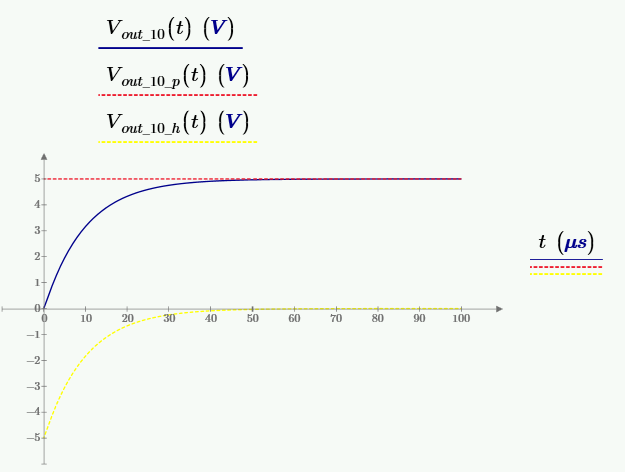
\includegraphics[height=5cm]{P_Fig/figur14_ana2graf10K}
  \caption{grafisk afbildning af $V_{out}{10}$}
  \label{graf10K}
 \end{center}
\end{figure}


